\section{LLM 请求调度的刻画}
\label{sec:principles}

\begin{figure*}[!t]
    \hspace{1mm}
     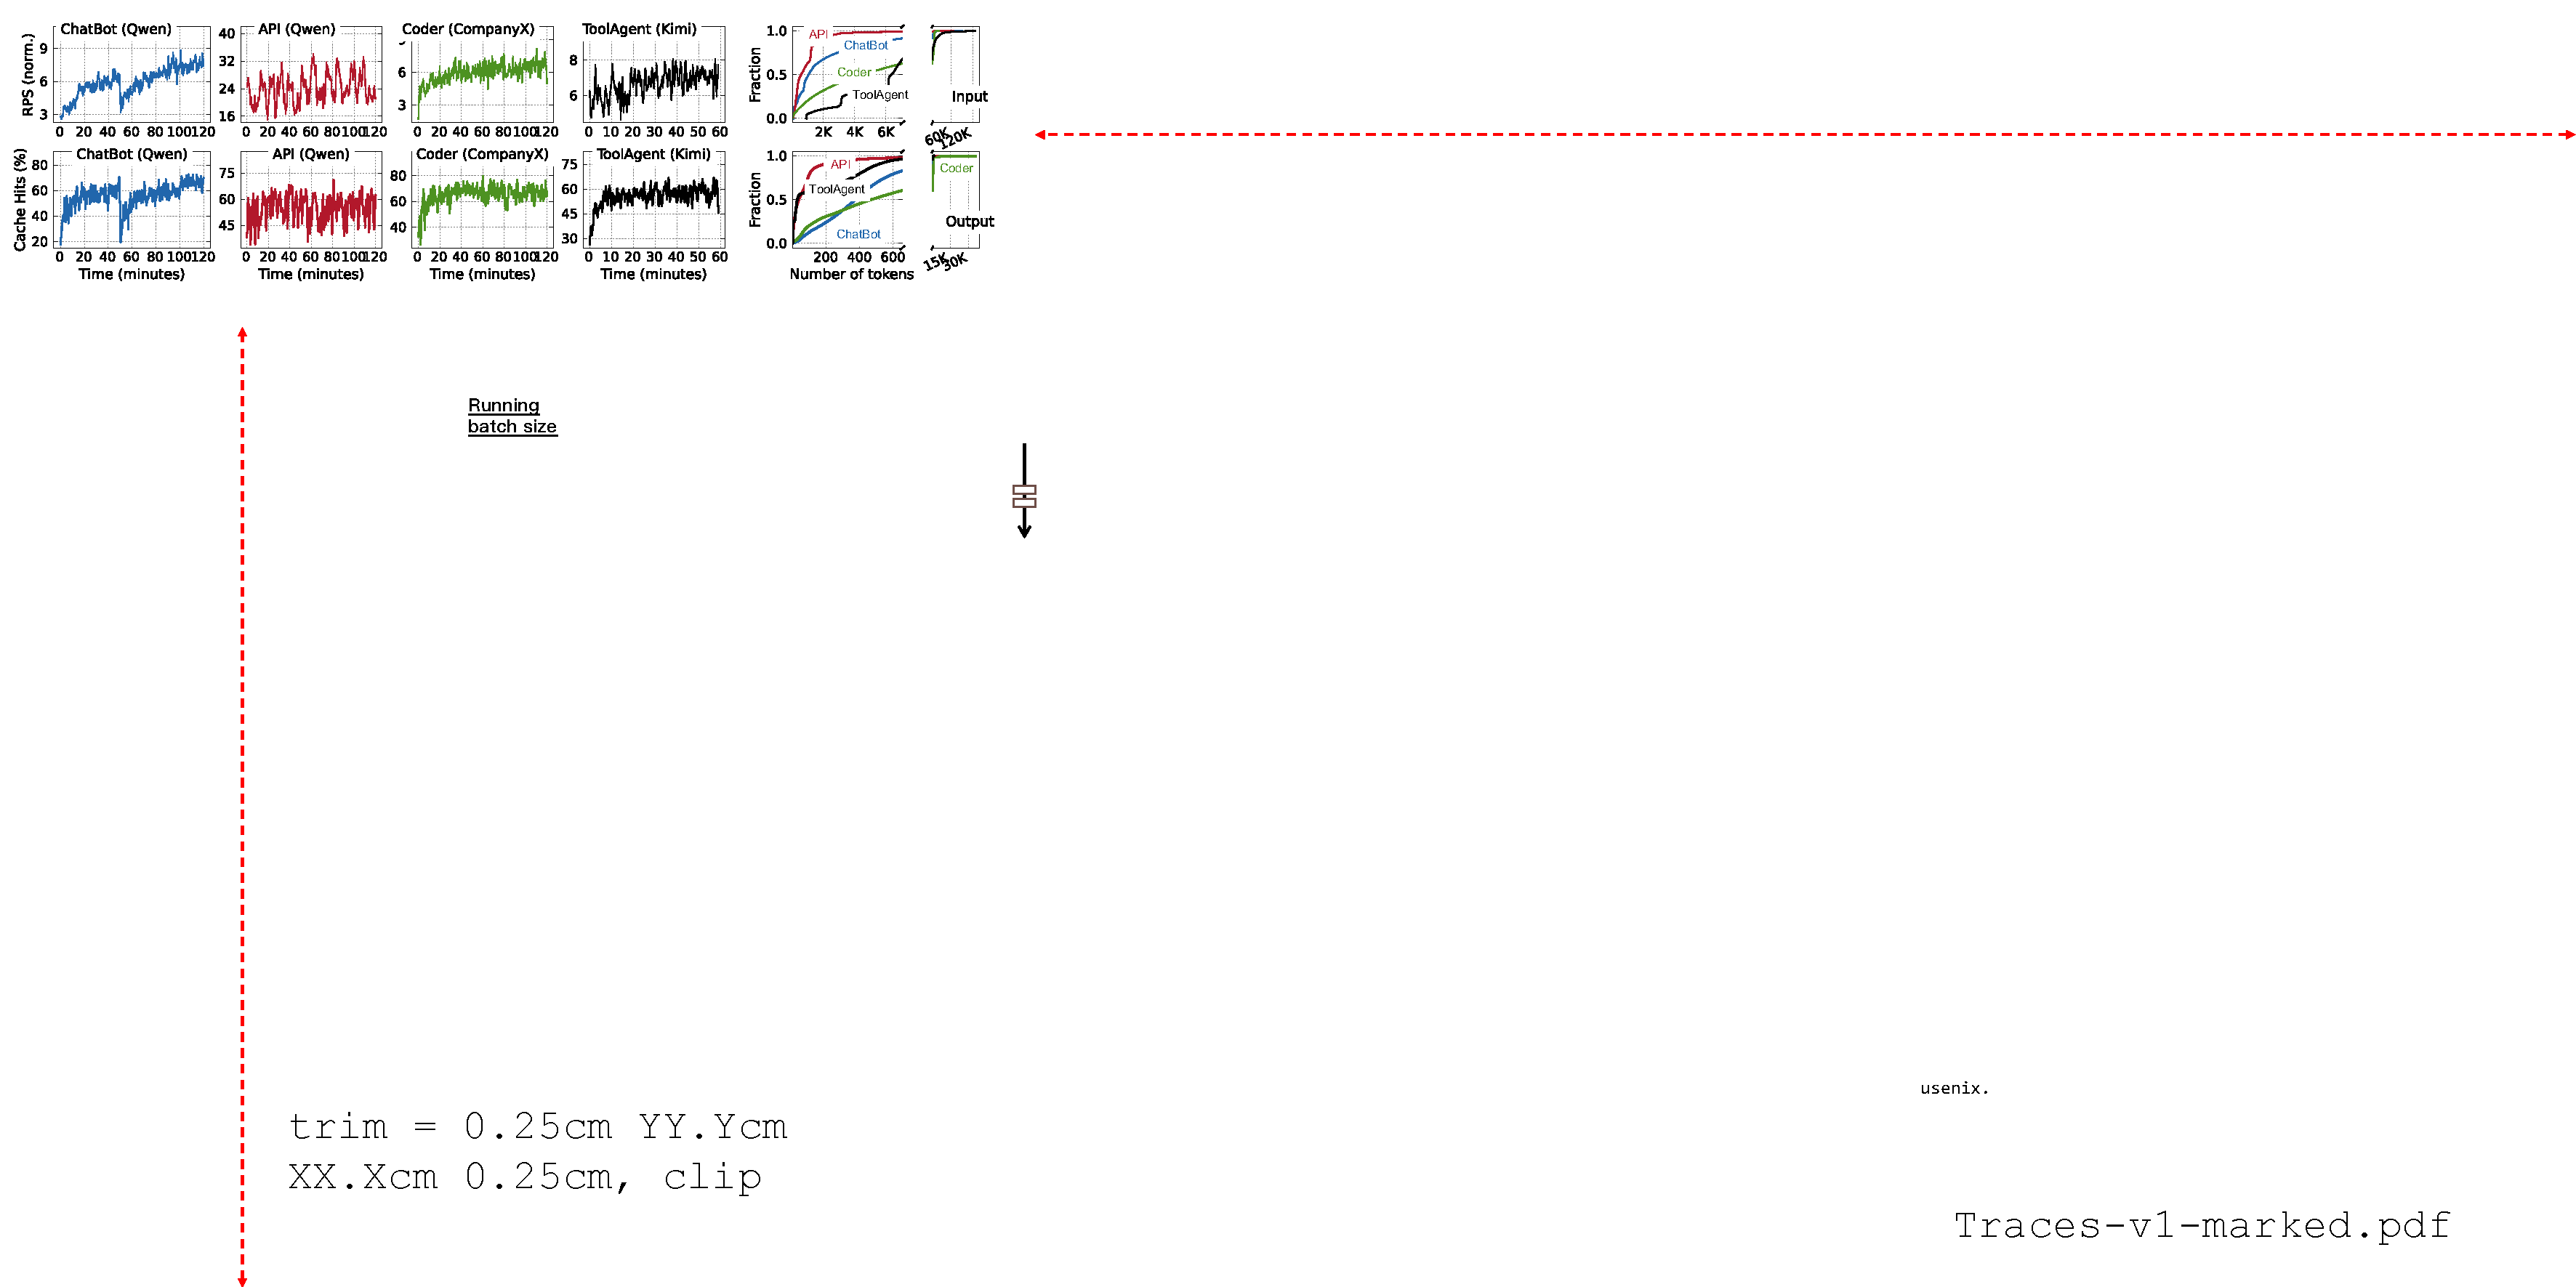
\includegraphics[width=0.99\linewidth, trim=0.25cm 22.45cm 36cm 0.25cm, clip]{figs/motiv/traces-v1-marked.pdf} \\[-18pt]
    \begin{minipage}{1\linewidth}
    \caption{\small{%
       本文研究的轨迹，覆盖了支撑 LLM 服务的主要场景。
        }}
    \label{fig:traces}
    \end{minipage} \\[-14pt]
\end{figure*}

\subsection{刻画方法}
\label{sec:eval-setup}

\nospacestitle{测试床与实例配置。\,}
除非特别说明，本文所有实验都在一个包含 16 张 NVIDIA H20 GPU 的测试床上进行——该硬件与 {\company} 用于承载 LLM 服务的硬件相近。
每张 GPU 具有 96\,GB HBM，足以承载市场上常见的模型~\cite{DBLP:conf/sosp/Xiang0QYZYZL0025}。
路由器部署在一台高端 CPU 服务器上，配备 160 个 Intel Xeon 核心和 1\,TB DRAM。
我们的实例运行最新的 vLLM-v1（vLLM）~\cite{vllm-code}——当前最先进的 LLM 服务引擎之一，并包含 chunked prefill~\cite{298679} 与快速 GPU kernel~\cite{flashinfer} 等最新优化。

\stitle{模型。\,}
我们选择了具有代表性的、且在市场上广泛使用的 LLM 模型，覆盖不同架构，包括稠密模型（Qwen2-7B）和混合专家模型（MoE，Qwen3-30B）~\cite{DBLP:conf/sosp/Xiang0QYZYZL0025}。

\stitle{工作负载。\,}
我们在真实世界的 LLM 服务轨迹上开展分析，这些轨迹既包括开源数据，也包括来自 {\company} 的内部采样，并覆盖了常见的 LLM 应用：
\textbf{ChatBot (Qwen)} 和 \textbf{Agent (Qwen)}~\cite{bailian}
是阿里云开源的轨迹，分别采集自类似 ChatGPT 的聊天机器人服务以及 LLM API 调用型智能体服务~\cite{claudeapi,geminiapi,openaiapi}；
\textbf{Coder} 收集了 {\company} 某代码 copilot 服务在 2025 年 11 月某一天发往专用集群的请求；
而 \textbf{ToolAgent (Kimi)}~\cite{mooncake-trace} 是另一份来自 Kimi 的开源轨迹，同样采集自智能体服务。
除 ToolAgent (Kimi) 外，其余轨迹都来自单个由一个全局路由器管理的集群；ToolAgent (Kimi) 未说明具体采集方式。

我们所分析的工作负载具有代表性——不仅因为场景覆盖面广，还因为每条轨迹都保留了评估 LLM 调度策略所需的关键特征。
具体来说，所有请求都包含请求内容的（哈希后）信息以及请求发起时间戳，这对于评估 {\kvcache} 感知调度对全局调度的影响至关重要（见 \textsection{\ref{sec:kvcache-aware}}）。
其他流行数据集，如 AzureLLMTrace~\cite{AzurePublicDataset} 或 BurstGPT~\cite{wang2025burstgpt}，并不提供这类内容信息。
需要注意的是，即使轨迹中只保存了哈希后的内容，我们仍然可以根据哈希值重建输入，从而以与原始轨迹完全一致的行为进行回放；
此外，无论 EOS token 如何，各实例执行的解码次数都与轨迹中记录的一致~\cite{kvcache}。

{\fig{fig:traces}} 可视化了这些轨迹的关键特征，包括请求到达率、输入与输出 token 数，以及假设 {\kvcache} 空间无限时的 {\kvcache} 命中率。
由于保密要求，\textbf{Coder} 轨迹中的请求到达率经过了归一化处理。
在所有这些轨迹上，我们都观察到：在给定的服务时间区间（例如 1 小时）内，请求到达率和 {\kvcache} 命中率整体较为稳定，仅存在少量短时波动。
此外，尽管不同轨迹的输入和输出 token 数存在差异，但除了极少数离群点之外，它们通常都不算特别大。

\stitle{轨迹缩放。\,}
由于这些轨迹最初采集自与我们测试床规模不同的集群，我们参考既有工作~\cite{DBLP:conf/asplos/MiaoSDXL0J24,DBLP:journals/pvldb/AliPYS22,DBLP:conf/osdi/GujaratiKAHKVM20,DBLP:conf/osdi/ZhangWLWS0025,traceupscaler}，按照测试床能力对轨迹进行缩放。
除非特别说明，我们将平均请求到达率缩放到通过离线分析得到的测试床最大处理速率的一半。
这与 {\company} 的实际服务配置相近，因为如果到达率逼近服务能力，{\company} 常见的做法是将请求重定向到另一个负载较低的集群，或者在非关键场景（如 ChatAPP）下直接拒绝部分请求~\cite{305212}。
否则，由于排队，大量请求的服务级目标（SLO）将无法满足~\cite{queuing}。
我们在 \textsection{\ref{sec:eval}} 的端到端分析中还进一步测量了不同请求到达率对调度性能的影响，结果同样保持一致。


\subsection{仅靠负载均衡对 LLM 并不够}
\label{sec:kvcache-aware}

\begin{figure}[!t]
    \centering
     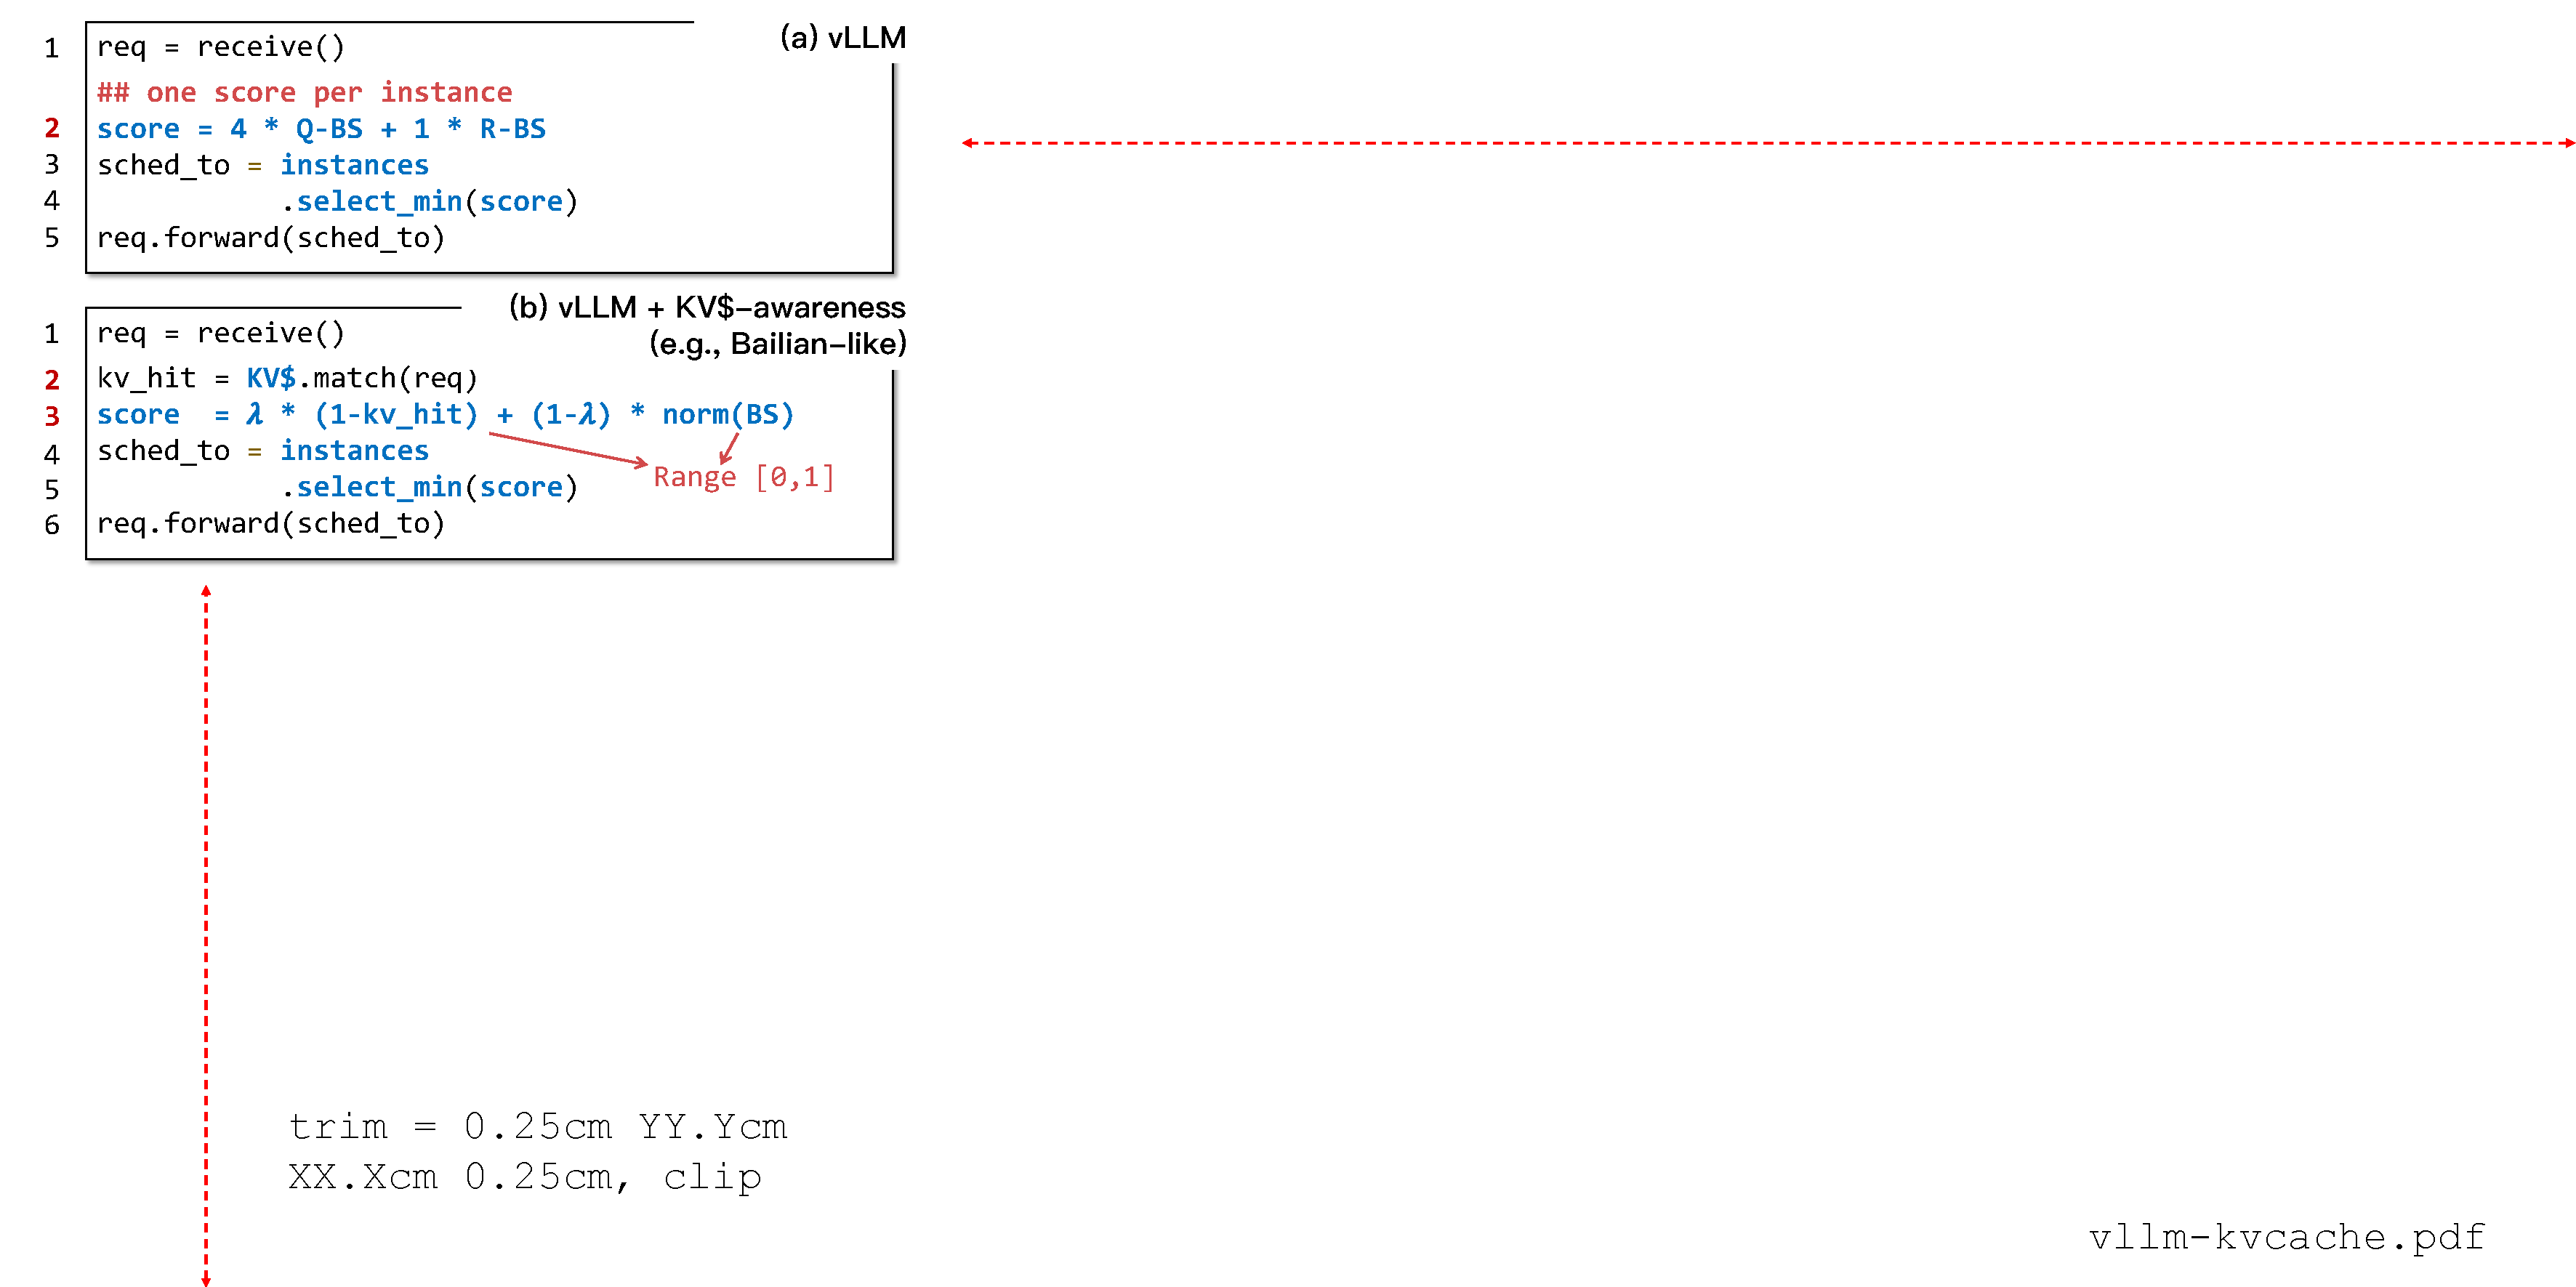
\includegraphics[width=0.9\linewidth, trim=0.25cm 16.4cm 37.65cm 0.25cm, clip]{figs/vllm-kvcache-v1.pdf} \\[5pt]
    \begin{minipage}{1\linewidth}
    \caption{\small{%
        (a) vLLM 的调度分数；
        以及 (b) 在其分数中加入 {\kvcache} 感知后的 LLM 调度方式。
        需要注意的是，两个指标的线性组合只有一个自由度（权重 $\lambda$）。
        }}
    \label{fig:vllm-kvcache}
    \end{minipage} \\[-10pt]
\end{figure}

\begin{figure}[!t]
    \centering
    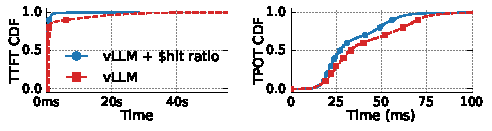
\includegraphics[width=1.0\linewidth]{figs/4-2-kvcache-aware/4-2-kvcache-aware-cdf-1-no-tail.pdf} \\[-0pt]
    \begin{minipage}{1\linewidth}
    \caption{\small{   
        在 Qwen3-30B 模型与 ChatBot 轨迹上，vLLM 与 KV cache 感知调度的性能对比。
        其他工作负载和模型也呈现类似趋势。
    }}
    \label{fig:kvcache-aware-cdf-1}
    \end{minipage} \\[-10pt]
\end{figure} 

\begin{figure}[t]
    \centering
    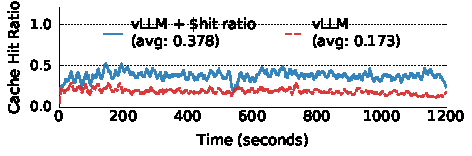
\includegraphics[width=0.97\linewidth]{./figs/4-2-kvcache-aware/kvcache-hit-timeline.pdf} \\[0pt]
    \begin{minipage}{1\linewidth}
    \caption{\small{Qwen3-30B 模型在 ChatBot 轨迹上的 {\kvcache} 命中率对比：vLLM vs. {\kvcache} 感知调度。
    其他工作负载和模型也类似。
    }}    
    \label{fig:kvcache-aware-hit-ratio1}
     \end{minipage} \\[-5pt]
\end{figure}


\begin{figure}[t]
    \centering
    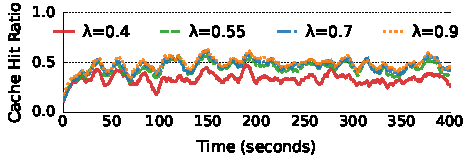
\includegraphics[width=0.97\linewidth]{figs/4-3-imbalance/4-2-cache-hit-t.pdf} \\[1pt]
     \begin{minipage}{1\linewidth}
    \caption{\small{%
在 Qwen3-30B 模型与 ChatBot 轨迹上，改变 {\kvcache} 感知项权重时，
策略（{\fig{fig:vllm-kvcache}} (b)）的 {\kvcache} 命中率对比。     
    }}
    \label{fig:chln-cache-hit}
    \end{minipage}
\end{figure}

\begin{figure}[!ht]
    \centering
    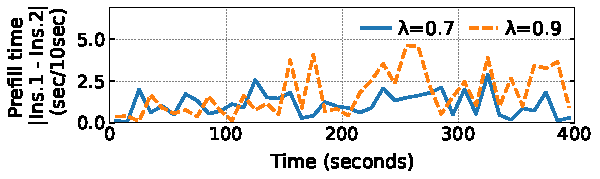
\includegraphics[width=0.98\linewidth]{figs/4-3-imbalance/4-3-pt-imbalance-absdiff.pdf} \\[-2pt]
    \caption{\small{%
    在 ChatBot 轨迹与 Qwen3-30B 模型上，使用两种不同线性组合权重运行时，两台实例之间工作负载失衡情况的剖面图。
    图中报告的指标是在每个 10 秒时间窗内，两台实例（Inst.）已服务预填充时间的绝对差值。
    }}
    \label{fig:chln-pt-imbalance}
\end{figure}

\nospacestitle{起点案例：vLLM 策略~\cite{vllm-code}。\,}
我们的研究从 vLLM~\cite{vllm-code} 采用的默认全局调度策略开始——它是工业界与学术界都广泛使用的流行开源 LLM 服务引擎。
{\fig{fig:vllm-kvcache}} (a) 展示了其调度方法：它使用每个实例的批大小作为路由分数的指标。
本质上，它是经典“最短队列优先”（join-the-shortest-queue, JSQ）负载均衡策略在 LLM 场景下的一个变体：对每个实例而言，批大小同时包含正在该实例上运行的请求数（R-BS）和在实例队列中等待的请求数（Q-BS）。

\begin{figure*}[!t]
    \centering
     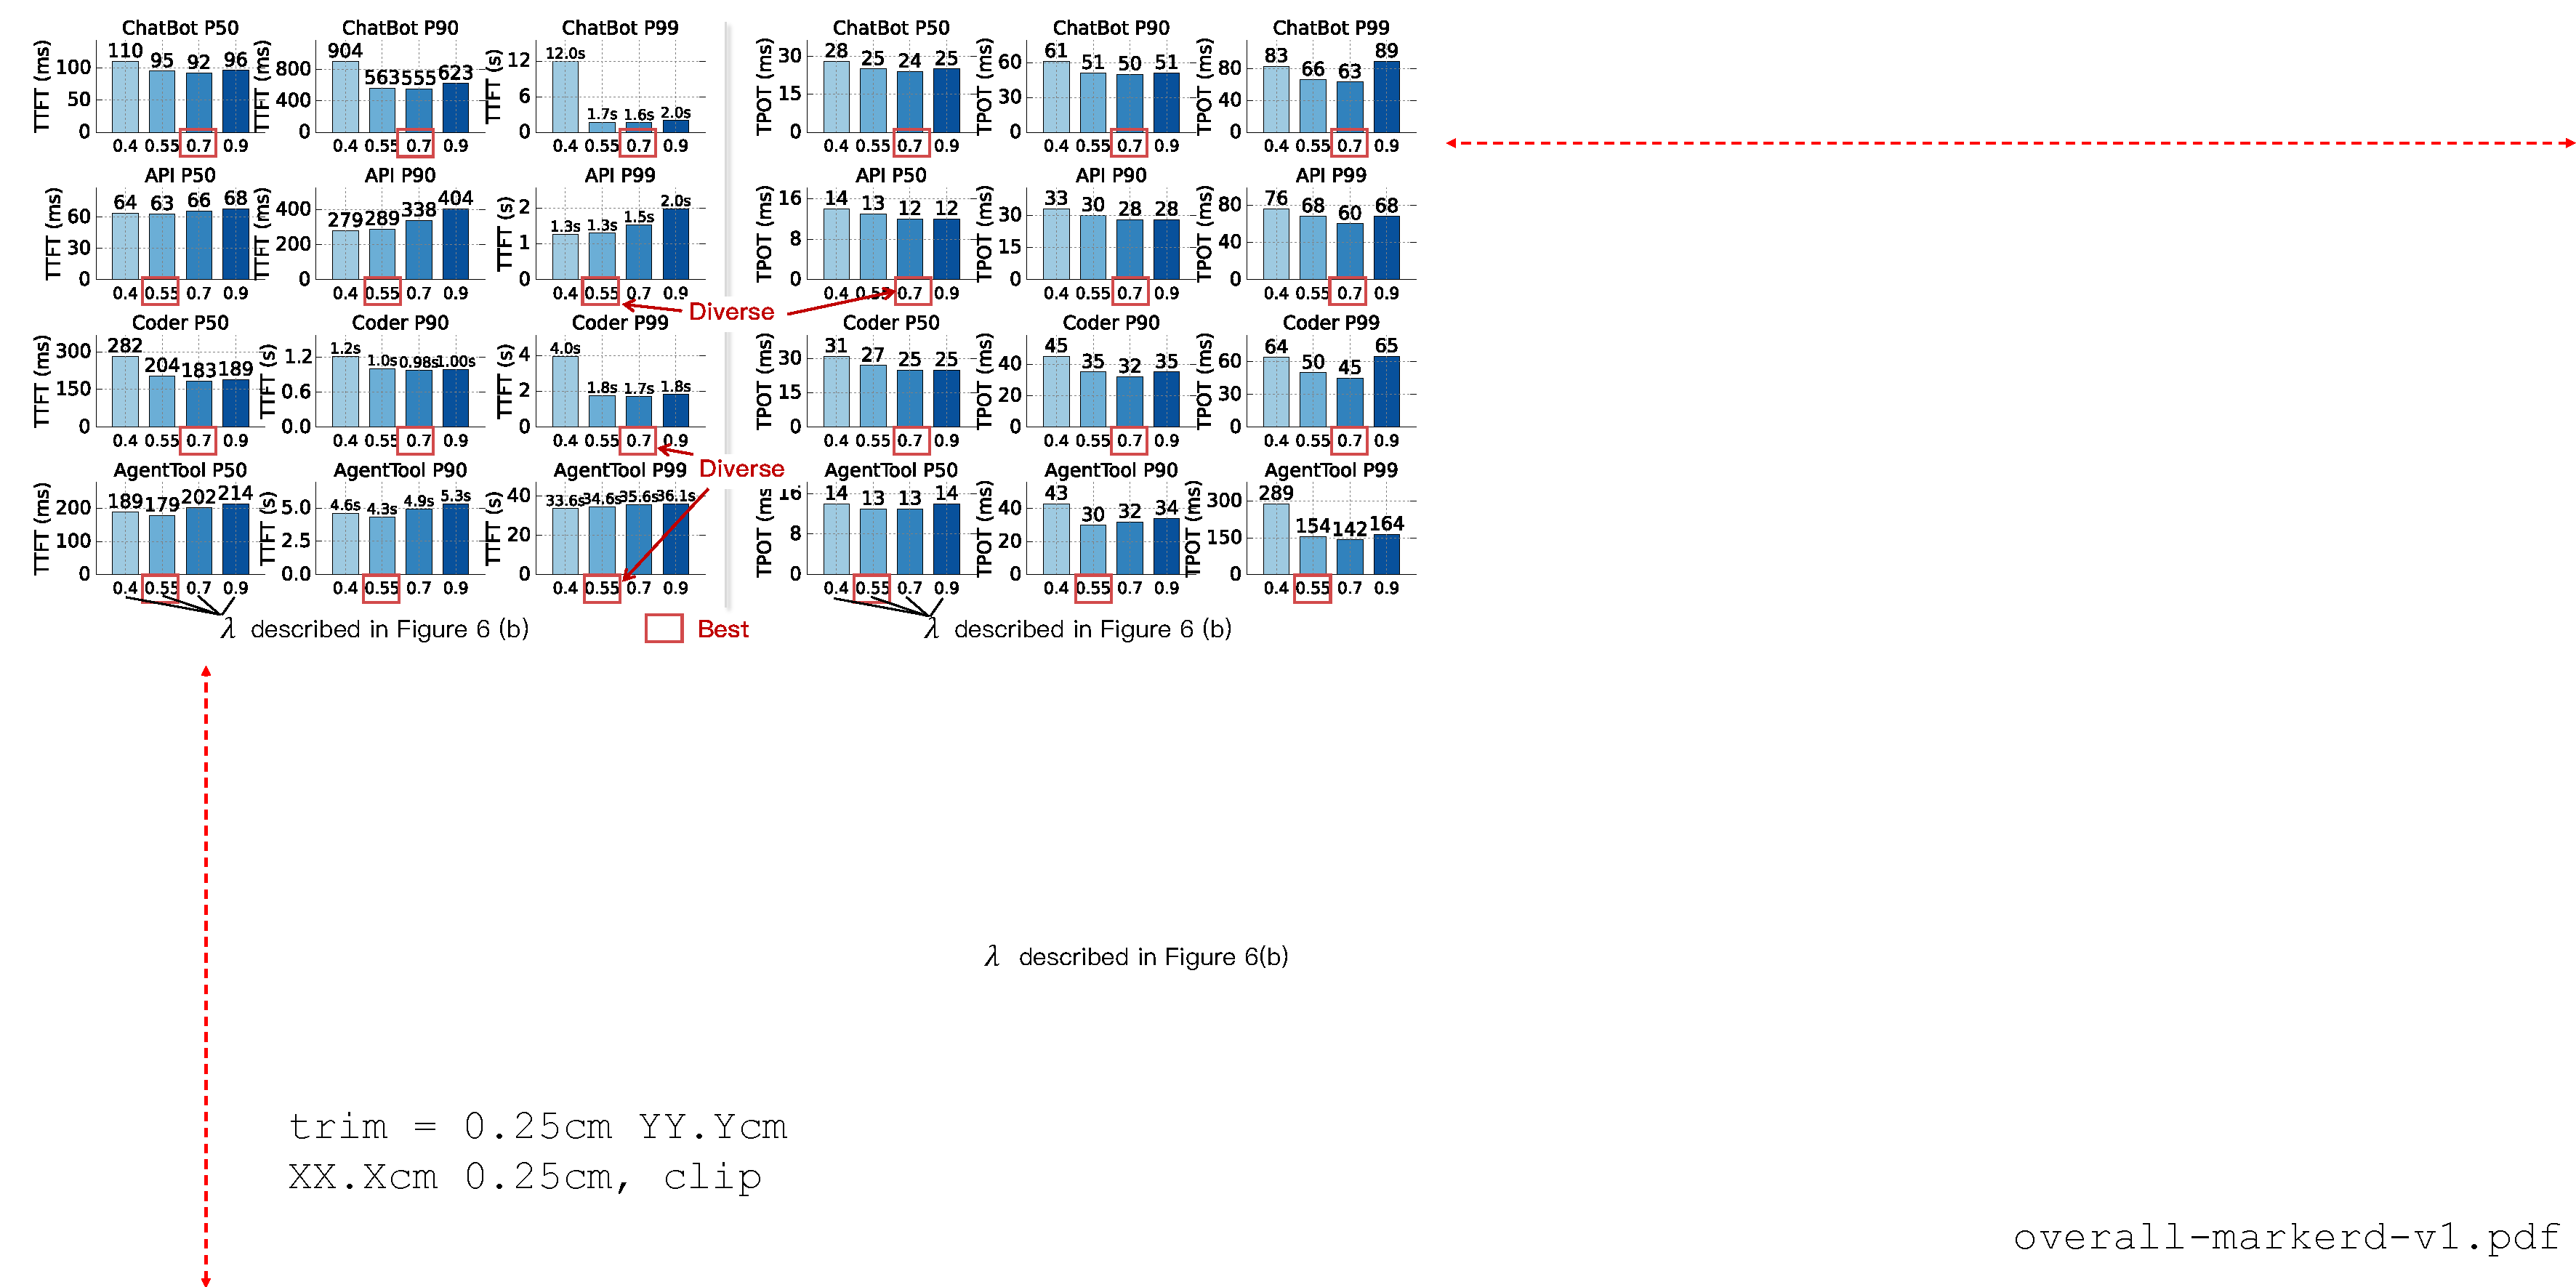
\includegraphics[width=0.95\linewidth, trim=0.25cm 14.52cm 26.5cm 0.25cm, clip]{figs/lambda-bar-chart/overall-marked-v1.pdf} \\[0pt]
    \begin{minipage}{1\linewidth}
    \caption{\small{%
        在线性组合方法下，不同超参数对四条轨迹性能的影响分析。
        所用模型为 Qwen3-30B。
        }}
    \label{fig:data-linear-tune}
    \end{minipage} \\[-10pt]
\end{figure*}

\stitle{为 vLLM 加入 {\kvcache} 感知（{\company}）。\,}
虽然 JSQ 尝试在实例间均衡工作负载，但它并不知道新请求的 {\kvcache} 状态。
而事实上，将请求路由到具有更高 {\kvcache} 命中率的实例，可以显著降低请求时延。
{\fig{fig:vllm-kvcache}} (b) 展示了一种由 {\company} 及其他工作~\cite{ai-Dynamo,aigw} 采用的简单扩展方式，用来让请求调度具备 {\kvcache} 感知能力：
它在分数函数中加入了一个 {\kvcache} 指标——一个估计当请求被路由到某实例时 {\kvcache} 命中率的比率。
需要注意，$KV$ 是表示每实例 {\kvcache} 哈希映射的符号值。
这里有两点值得说明：
(1) 负载均衡指标（批大小）需要被归一化到 $[0,1]$，以匹配命中率的量纲，否则二者无法直接相加；
(2) 本节分析假设线性组合系数（$\lambda$）固定，而下一节将讨论如何设定这些系数。

正如 {\fig{fig:kvcache-aware-cdf-1}} 所示，
在仅做负载均衡的策略中加入 {\kvcache} 感知后，
平均 TTFT 提升了 84\%，平均 TPOT 提升了 17\%。
这符合预期，因为它提高了 {\fig{fig:kvcache-aware-hit-ratio1}} 所示的 {\kvcache} 命中率。
有趣的是，尽管更高的 {\kvcache} 命中率乍看之下似乎只会改善预填充阶段，
我们发现它也有助于降低解码时间，
因为它减少了每个实例所需的计算量，从而使实例能够把更多 GPU 时间分配给解码阶段。


\subsection{{\kvcache} 感知与负载均衡：二者的权衡}
\label{sec:challenge-balancing}

\noindent
尽管这一思路直观，但将 {\kvcache} 感知真正整合进系统并不简单。
根本原因在于，考虑 {\kvcache} 感知可能会干扰负载均衡。
具体而言，如前所述，当我们使用线性组合定义分数时，
两个目标的优先级由打分函数中各指标的权重控制（在 {\fig{fig:vllm-kvcache}} (b) 中为 $\lambda=0.4$）：
如果给 {\kvcache} 项分配更大的权重，
路由器就会优先把请求发往 {\kvcache} 命中率更高的实例，
即便其他实例的负载明显更低。
而这反过来又可能造成实例间的负载失衡。

{\fig{fig:data-linear-tune}} 通过展示不同 {\kvcache} 感知权重下、上一节所述线性组合策略（{\fig{fig:vllm-kvcache}} (b)）的整体 TTFT 与 TPOT，说明了这种权衡。
我们可以看到，当权重从 0.4 提升到 0.9 时，除 API 轨迹外，TTFT 都是先下降后上升；
API 轨迹受影响较小，这是因为其输入长度较短。

为了揭示这种权衡背后的原因，
{\fig{fig:chln-cache-hit}} 进一步展示了在 ChatBot 轨迹上改变 {\kvcache} 感知权重时的 {\kvcache} 命中率变化；其他轨迹也表现出类似趋势。
可以清楚地看到，随着 {\kvcache} 权重增加，整体 {\kvcache} 命中率也随之上升。
这解释了为什么当权重从 0.4 增加到 0.7 时，TTFT 会下降。

尽管 {\kvcache} 命中率提高了，但在某个权重拐点之后（例如 ChatBot 上的 0.7），整体时延反而开始上升。
这源于实例间的负载失衡；我们在 {\fig{fig:chln-pt-imbalance}} 中刻画了这一现象。
该图展示了在同一个 400 秒突发区间内，使用两种不同线性组合权重（0.7 vs. 0.9）服务同一条 ChatBot 轨迹时，两台实例所承担的预填充工作量。
这里的预填充时间指每个 10 秒时间窗内，该实例用于预填充的总秒数。
这是衡量实例工作负载的一个良好指标，因为直观上大多数 token 都是在解码阶段生成的；因此，如果某个实例的处理时间被预填充主导，那么它生成的 token 数通常就会少于其他实例。
为便于展示，我们从总共 16 台实例中选取预填充时间标准差最高的两台。
我们观察到，当 {\kvcache} 优先级更高（$\lambda=0.9$）时，这两台实例的总预填充时间差异非常明显。
相比之下，在较为均衡的设置（$\lambda=0.7$）下，两台实例的预填充时间相近，而且这一时期的平均预填充时间也相近。
具体地说，在 $\lambda=0.7$ 时，两台实例的平均预填充时间分别为 3.43s 和 3.40s；而在 $\lambda=0.9$ 时，则分别为 3.57s 和 2.17s。



\subsection{线性组合的情形}
\label{sec:linear-combination}

\noindent
基于前面对权衡关系的分析，
通过线性组合同时实现 {\kvcache} 感知和负载均衡，会带来两个问题：

\stitle{缺点 \#1：需要面向工作负载的超参数调优。\,}
{\kvcache} 的重要性及其对负载失衡的影响，都依赖于具体工作负载。
例如，{\fig{fig:data-linear-tune}} 给出了在 Qwen3-30B 模型下，不同轨迹的调参结果。
可以看到，不同工作负载的最优权重并不相同：
例如在 ChatBot 上最优权重是 0.7，而在 API 上则是 0.55，尽管它们的 {\kvcache} 访问模式相近。
需要注意的是，我们无法负担遍历所有可能配置的代价，因为在测试床上回放每一条轨迹都会消耗大量 GPU 时间。
因此，线性组合的性能依赖于面向具体工作负载的超参数调优，而在实践中，由于工作负载高度多样，这种调优并不容易~\cite{10.5555/3768039.3768067}。


\stitle{缺点 \#2：性能仍然可能次优。\,}
在 \textsection{\ref{sec:eval}} 的评估中，
我们发现，静态调好的权重并不总能取得与其他基线相竞争的性能。
我们推测，原因在于最优权重本身可能会随时间变化；
例如，不同请求的 {\kvcache} 命中模式就可能随时间变化（见 {\fig{fig:traces}} 的第二行）。
然而，据我们所知，现有所有工作都在整个服务期间使用一个固定的调优权重。
虽然理论上可以设计随时间自适应调权的策略，但这会进一步增加系统复杂度。

\begin{figure*}[!t]
    \centering
     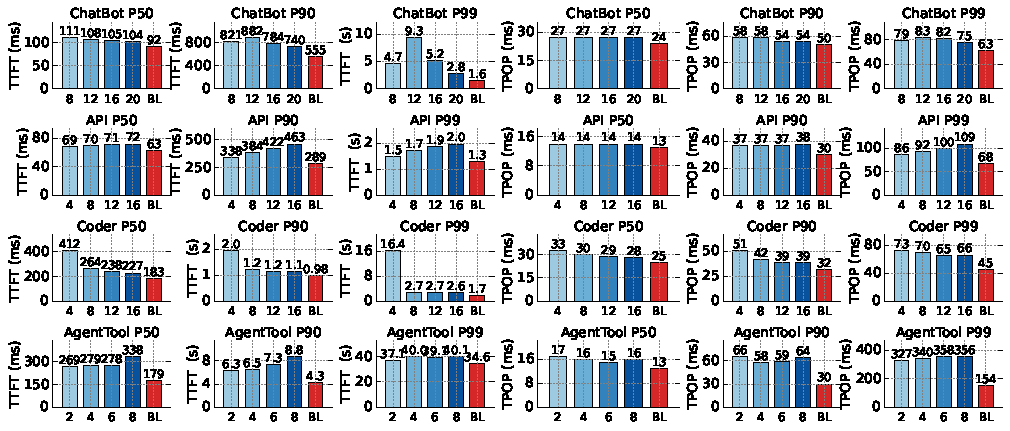
\includegraphics[width=0.99\linewidth]{figs/filter-based/overall-v1.pdf} \\[2pt]
    \begin{minipage}{1\linewidth}
    \caption{\small{%
        在基于过滤的组合方法下，不同超参数对四条轨迹性能的影响分析。
        \textbf{BL} 表示用于对比的\uline{线}性组合方法，其超参数已调到\uline{最优}。
        图中的数字（2,4,6,8）对应 {\fig{fig:aibrix}} 中描述的范围。
        所用模型为 Qwen3-30B。
        }}
    \label{fig:data-filter-tune}
    \end{minipage} \\[-10pt]
\end{figure*}

\subsection{基于过滤组合的情形}
\label{sec:filter-combination}

\begin{figure}[!t]
    \centering
     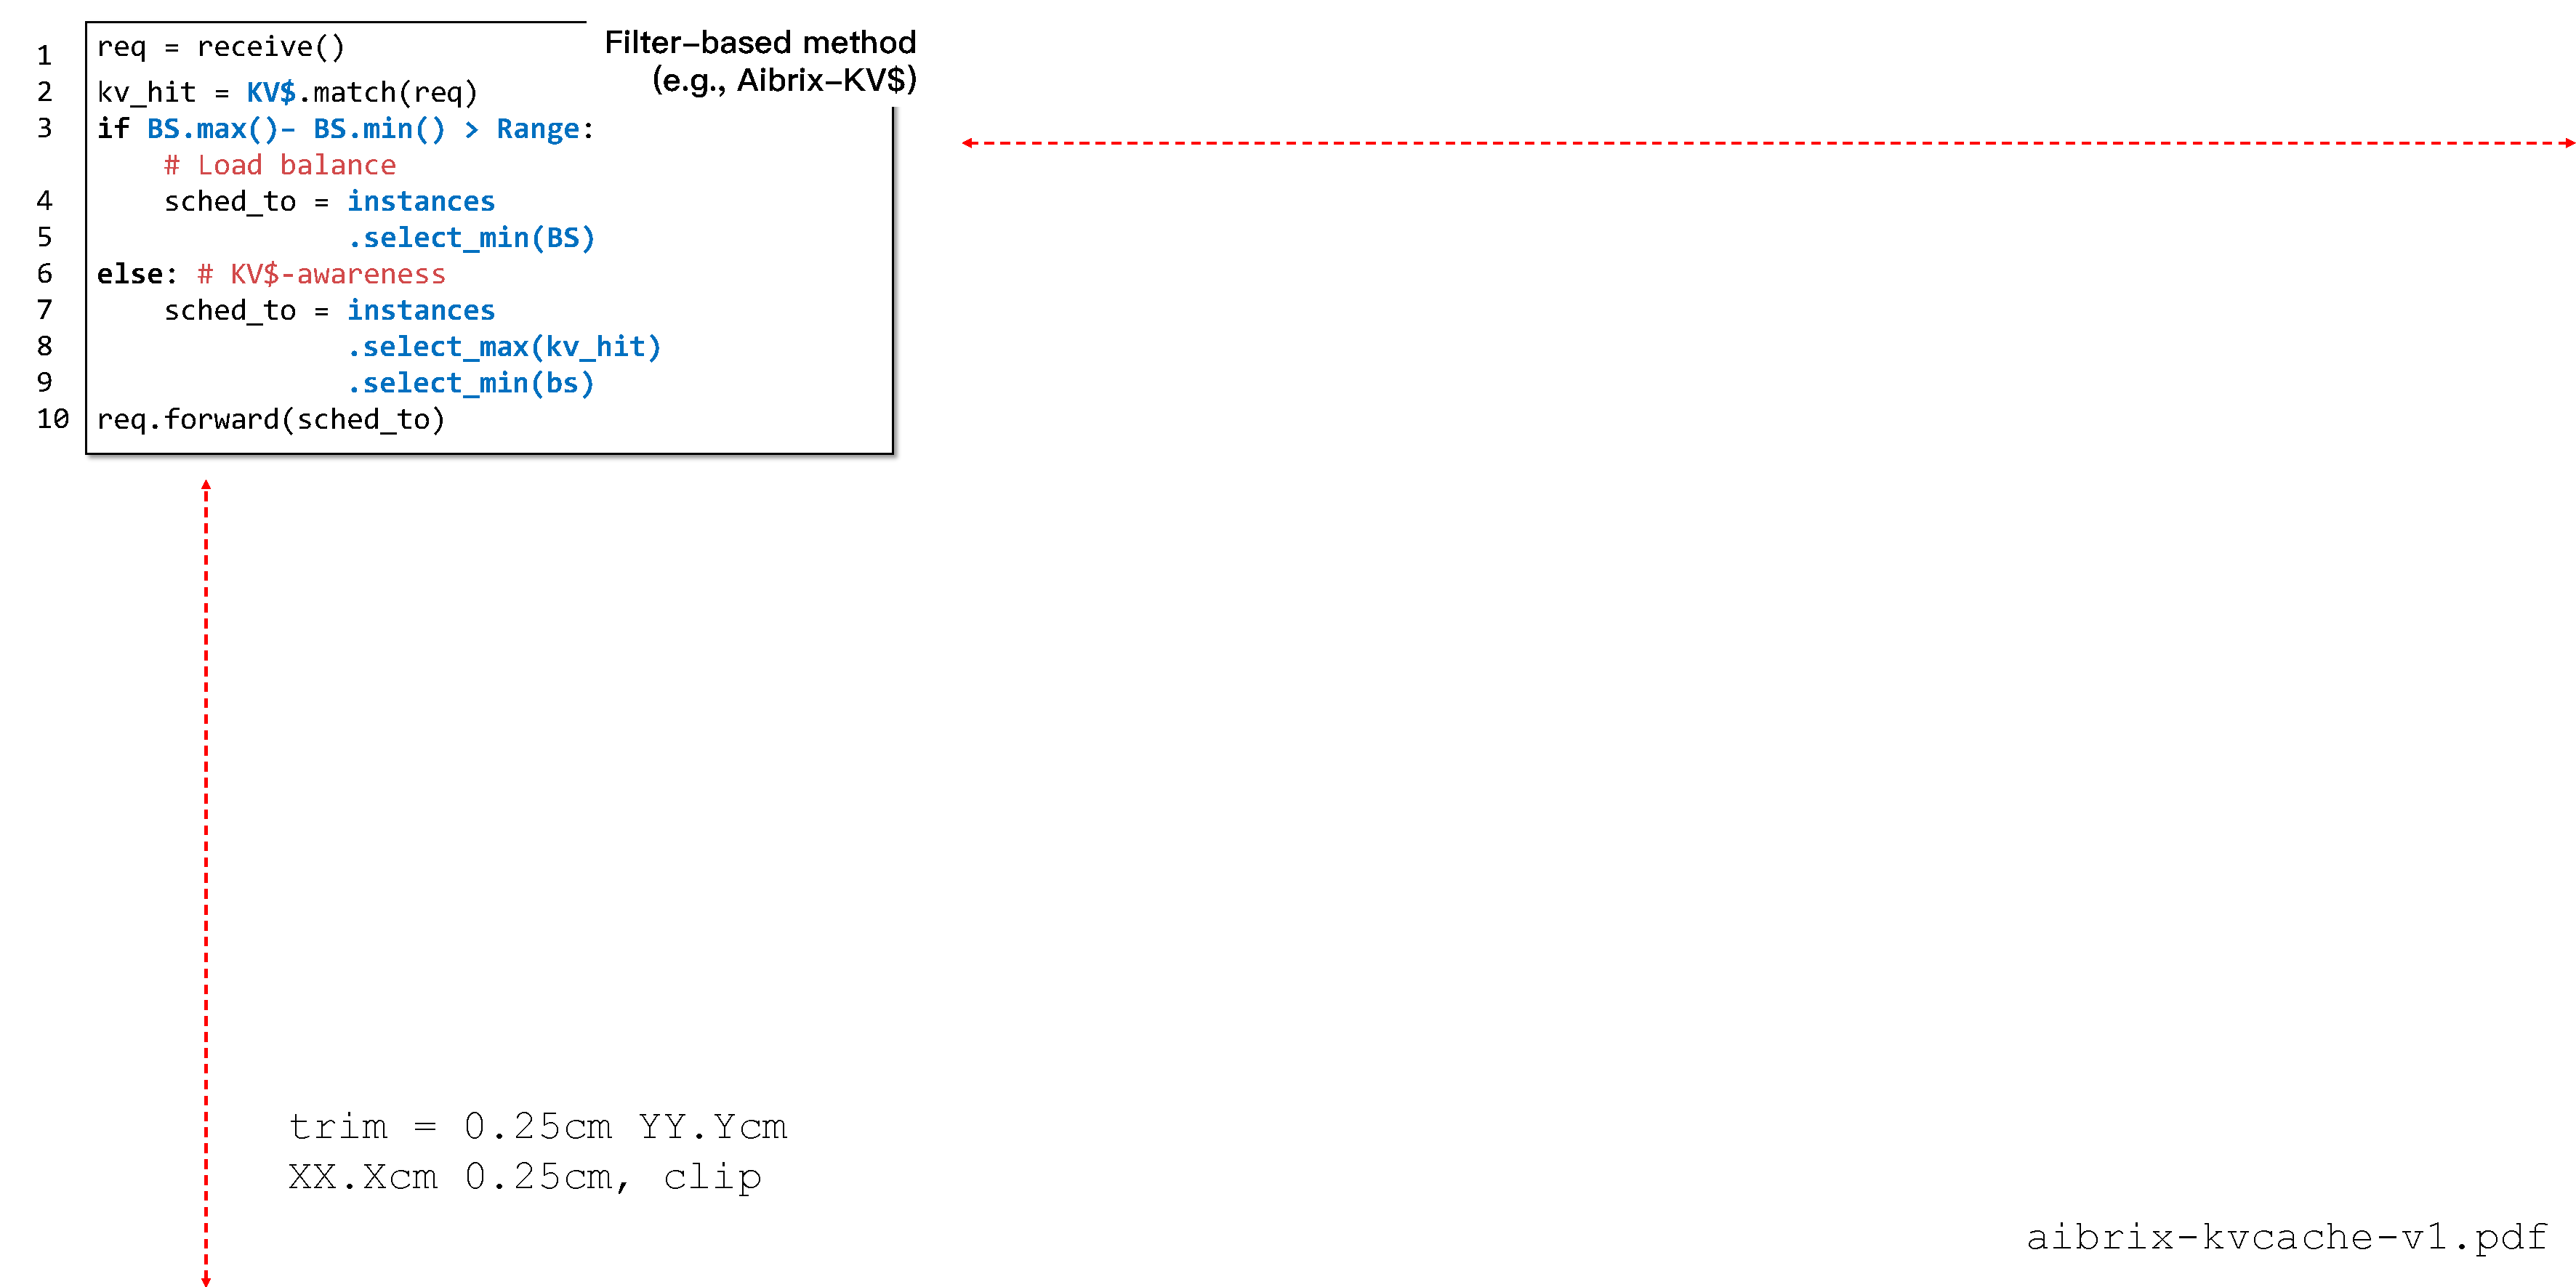
\includegraphics[width=0.9\linewidth, trim=0.25cm 18.9cm 37.65cm 0.25cm, clip]{figs/aibrix-kvcache-v1.pdf} \\[5pt]
    \begin{minipage}{1\linewidth}
    \caption{\small{%
        在 LLM 调度中，将 {\kvcache} 感知与负载均衡结合的基于过滤方法伪代码，
        由 AIBrix~\cite{aibrix} 的 \texttt{prefix-cache} 策略简化而来。
        }}
    \label{fig:aibrix}
    \end{minipage} \\[-10pt]
\end{figure}

\nospacestitle{方法。\,}
{\fig{fig:aibrix}} 展示了在 AIBrix~\cite{aibrix} 等典型 LLM 调度系统中，
一种将 {\kvcache} 感知与负载均衡结合起来的典型过滤式方法。
首先，路由器会检查当前集群是否负载失衡——即所有实例间最大批大小与最小批大小之差（\(\texttt{BS.max() - BS.min()}\)）是否超过某个阈值（第 3 行）。
如果超过，路由器就放弃 {\kvcache} 感知，直接把请求路由到批大小最小的实例，以恢复负载均衡（第 4--5 行）。
否则，路由器使用 {\kvcache} 命中率这一指标，在实例之间进行选择（第 6--9 行），从而实现 {\kvcache} 感知。

\stitle{缺点 \#1：仍然需要面向工作负载的超参数调优。\,}
与线性组合类似，基于过滤的方法同样需要调参，因为用于判断负载失衡的阈值（\texttt{Range}）依赖于具体工作负载。
正如 {\fig{fig:data-filter-tune}} 所示，某个典型过滤方法~\cite{aibrix} 的最优阈值会随工作负载而变化：
例如在 Coder 轨迹上，将阈值从 4 提升到 16，可以分别改善 44\% 的 P50 TTFT 和 15\% 的 TPOT；
而在 API 轨迹上，16 又明显优于 4。


\stitle{缺点 \#2：性能仍然次优。\,}
除了需要调参之外，基于过滤的组合方法通常也比调到合适权重的线性组合更慢，如 {\fig{fig:data-filter-tune}} 所示。
这是因为它偏向负载均衡，可能放弃了 {\kvcache} 感知带来的收益。
更具体地说，一旦检测到负载失衡，它就会完全忽略 {\kvcache} 感知；
但在某些情况下，即使存在一定失衡，把请求路由到具有更高 {\kvcache} 命中率的实例仍可能是有益的，
因为显著减少的计算量本身也有助于缓解负载。
在线性组合中，只要分配给 {\kvcache} 命中率的权重不太小，这一点是可以做到的；
而基于过滤的方法无法表达这种折中。

\subsection{基于模拟组合的情形}
\label{sec:prediction-combination}
\begin{figure}[!t]
    \centering
     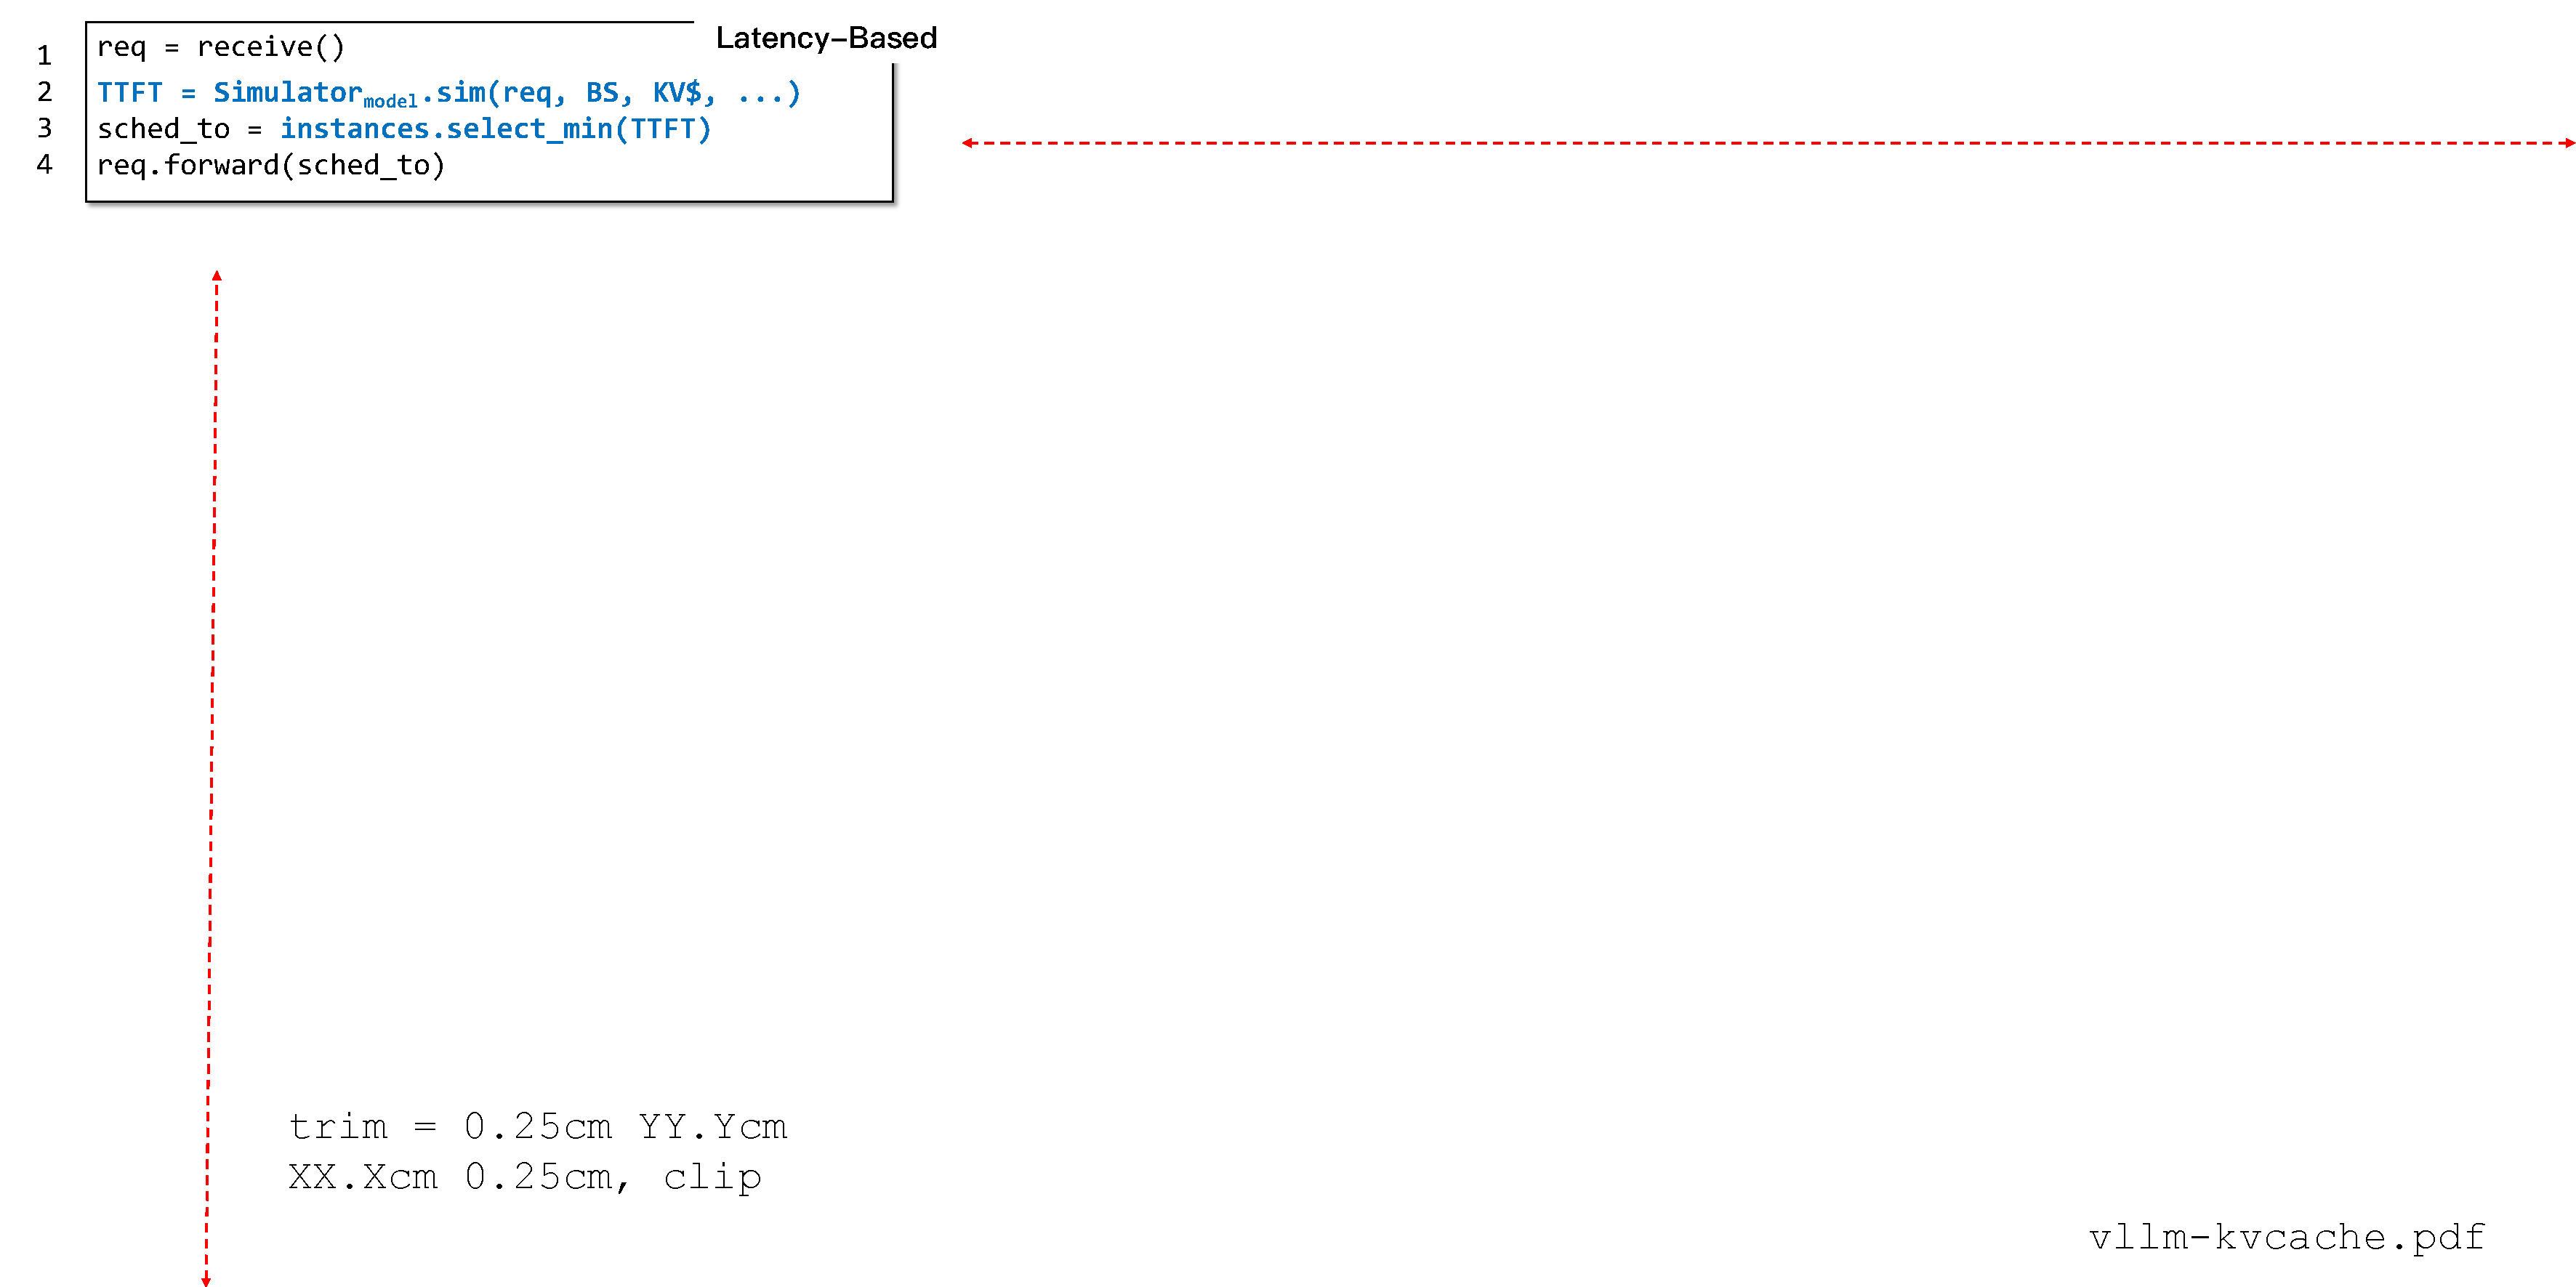
\includegraphics[width=0.96\linewidth, trim=0.25cm 25cm 38cm 0cm, clip]{figs/latency-based-v1.pdf} \\[6pt]
    \begin{minipage}{1\linewidth}
    \caption{\small{%
        在 LLM 调度中，将 {\kvcache} 感知与负载均衡结合起来的基于模拟方法伪代码。
        }}
    \label{fig:latency-based-scheduling}
    \end{minipage} \\[-10pt]
\end{figure}


\begin{figure*}[!t]
    \centering
    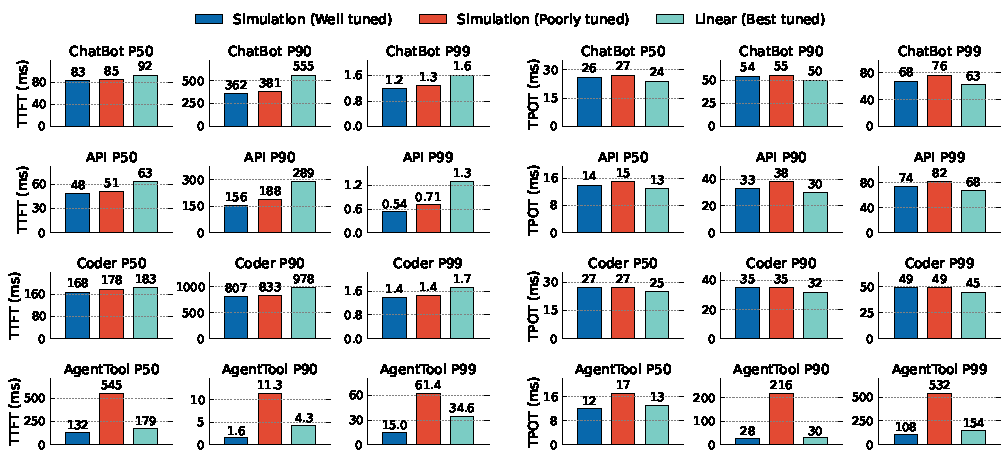
\includegraphics[width=0.85\linewidth]{figs/tuning/predictor-vs-wrong-predictor-v3.pdf} \\ 
    \begin{minipage}{1\linewidth}
    \caption{\small{%
    在 Qwen3-30B 模型上，不同模拟器准确度对四条轨迹性能影响的分析。
        }}
    \label{fig:wrong-predictor-e2e}
    \end{minipage} \\[-10pt]
\end{figure*}

\begin{figure}[t]
    \centering
    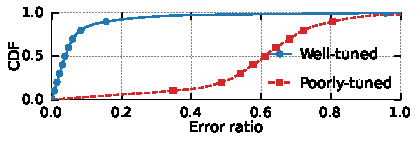
\includegraphics[width=0.85\linewidth]{figs/tuning/predictor-vs-wrong-predictor-accuracy.pdf} \\[-5pt]
    \caption{\small{   
    在 Qwen3-30B 模型与 ChatBot 轨迹上，调优良好的模拟器与未调优模拟器的对比。
    }}
    \label{fig:predictor-accuracy-cdf}
\end{figure}

\nospacestitle{方法。\,}
最后，基于模拟的方法~\cite{305212, llm-d, DBLP:journals/corr/abs-2507-17769, DBLP:journals/corr/abs-2504-08784}
会把“请求被路由到某个实例后，其模拟服务时间”作为路由分数。
这一思路基于这样一个观察：LLM 请求的执行过程高度结构化，因此可以较准确地模拟。
{\fig{fig:latency-based-scheduling}} 展示了一种典型模拟式方法~\cite{llm-d} 的伪代码：
在接收到请求后，路由器先通过模拟器（例如 VIDUR~\cite{DBLP:conf/mlsys/AgrawalKMPKGRT24}）估计请求路由到每个实例后的 TTFT（第 2 行），
然后把请求发送到估计 TTFT 最低的实例（第 3--4 行）。
需要注意的是，这类方法通常只估计 TTFT，而不是端到端时延，因为端到端时延还取决于输出 token 数，而这是不可预测的。

基于模拟的解决方案可以被看作是一种更高阶的指标组合方式，
因为为了准确模拟 TTFT，模拟器必须把每个实例的 {\kvcache} 状态和批大小作为输入特征。
在这里，我们选择了一个与 llm-d~\cite{llm-d} 类似的模拟式实现，
但将其中的模拟器替换为改造后的 VIDUR~\cite{DBLP:conf/mlsys/AgrawalKMPKGRT24}——这是当前最先进的 LLM 实例模拟器。
我们的改造包括两部分：
(1) 扩展模拟器，使其在模拟预填充阶段时考虑带缓存命中的 {\kvcache} 感知执行；
(2) 用 Rust 重新实现它，并启用并行模拟，以便在线上支持跨多个实例的模拟调度。
如果不考虑 {\kvcache} 感知，模拟式方案就无法超越其他方法，这与我们在 \textsection{\ref{sec:kvcache-aware}} 中的观察一致。
如果不使用 Rust，原始的 Python 实现会带来明显的调度延迟，并不适合在线调度。
我们还做了若干优化，使模拟器能够扩展到数百个实例；不过这些内容并非本文重点，将留待后续论文展开。

我们研究了一种最先进的方法，发现它在某些轨迹上优于线性组合方法，这一点也在 {\fig{fig:latency-based-scheduling}} 中有所体现。
尽管性能有所提升，基于模拟的方法由于其复杂性，仍存在两个问题：

\stitle{缺点 \#1：由于按模型开发和按硬件调优带来的开发复杂度。\,}
基于模拟的方法性能高度依赖模拟器的准确性，而要在实践中达到高准确度并不容易，
因为我们既要考虑模型架构，又要考虑硬件特性。
为了量化模拟器准确度对调度性能的影响，
{\fig{fig:wrong-predictor-e2e}} 给出了在 Qwen3-30B 模型上，使用“调优良好”与“未调优”模拟器时四条轨迹的性能对比。
这里，“未调优”模拟器原本是为另一种模型——Qwen2-7B——设计的；而“调优良好”模拟器则是专门为 Qwen3-30B 实现的。
{\fig{fig:predictor-accuracy-cdf}} 进一步比较了这两个模拟器在服务 Qwen3-30B 时、相对 vLLM 的 TTFT 偏差。
可以看到，调优良好的模拟器准确度明显更高；
借助更准确的模拟器，TTFT 与 TPOT 的尾部时延可分别改善 75.6\% 和 79.7\%。

虽然可以为每种模型开发专门的模拟器，以换取更高的调度性能，
但这样会带来不小的开发复杂度，
因为模拟过程高度依赖模型架构，而模型架构又在快速演进，不断出现新模块（例如线性注意力~\cite{qwen3-next} 和 Engram~\cite{cheng2026conditionalmemoryscalablelookup}）。
与此同时，即便是同一个模型，模拟器的超参数也需要针对不同硬件特性重新调优，进一步增加了开发成本。

\stitle{缺点 \#2：性能仍然可能次优。\,}
基于模拟的方法仍会遭遇次优性能问题，尤其体现在 TPOT 上。
如 {\fig{fig:wrong-predictor-e2e}} 所示，在 AgentTool 轨迹上，它的 TPOT 尾时延比表现最好的线性组合方法高 71.1\%。
我们推测，这可能是因为模拟器的一些误判导致了负载失衡。
例如，在 {\fig{fig:predictor-accuracy-cdf}} 中可以看到，
即便使用调优良好的模拟器，仍有大约 10\% 的请求预测误差超过 20\%。
这类误差主要来自两个方面：vLLM API 服务器中的请求重排序，以及时延预测本身的不准确。
